\begin{figure}[H]
    \centering
    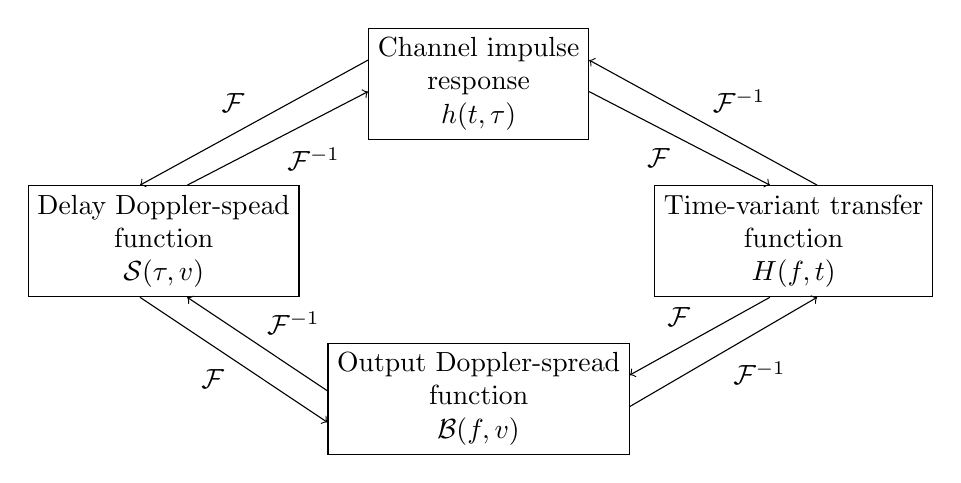
\begin{tikzpicture}
        \coordinate (center) at (0,0);
        \node[draw,align=center,above of=center,node distance=2cm] (impulse) {Channel impulse\\response\\$h(t,\tau)$};
        \node[draw,align=center,left of=center,node distance=4cm] (delay) {Delay Doppler-spead\\function\\$\mathcal{S}(\tau,v)$};
        \node[draw,align=center,below of=center,node distance=2cm] (output) {Output Doppler-spread\\function\\$\mathcal{B}(f,v)$};
        \node[draw,align=center,right of=center,node distance=4cm] (time) {Time-variant transfer\\function\\$H(f,t)$};

        \draw[<-] ([xshift=-.3cm]delay.north) -- ([yshift=+.3cm]impulse.west) node[midway,above left] {$\mathcal{F}$};
        \draw[->] ([xshift=+.3cm]delay.north) -- ([yshift=-.1cm]impulse.west) node[midway,anchor=north west] {$\mathcal{F}^{-1}$};

        \draw[->] ([xshift=-.3cm]delay.south) -- ([yshift=-.3cm]output.west) node[midway,below left] {$\mathcal{F}$};
        \draw[<-] ([xshift=+.3cm]delay.south) -- ([yshift=+.1cm]output.west) node[midway,above right] {$\mathcal{F}^{-1}$};

        \draw[->] ([xshift=-.3cm]time.south) -- ([yshift=+.3cm]output.east) node[midway,above left] {$\mathcal{F}$};
        \draw[<-] ([xshift=+.3cm]time.south) -- ([yshift=-.1cm]output.east) node[midway,anchor=north west] {$\mathcal{F}^{-1}$};

        \draw[->] ([xshift=+.3cm]time.north) -- ([yshift=+.3cm]impulse.east) node[midway,above right] {$\mathcal{F}^{-1}$};
        \draw[<-] ([xshift=-.3cm]time.north) -- ([yshift=-.1cm]impulse.east) node[midway,below left] {$\mathcal{F}$};
    \end{tikzpicture}
    \caption{Transfer functions of a frequency selective channel.}
    \label{fig:transfer_functions}
\end{figure}
